\chapter{Postproduktion}

In diesem Kapitel wird der Teil der Postproduktion beschrieben. Im Zusammenhang mit diesem Projekt ist dies das Zusammenführen von Filmmaterial und gerendertem Material im Schnitt, sowie das Nachbearbeiten dieser. Die Postproduktion ist in der Videoschnitt- und Farbkorrektursoftware DaVinci Resolve 16 geschehen.

\section{Schnitt}

Der erste Schnitt wurde vor der Produktion im Zusammenhang mit dem Animatic (siehe \autoref{sec:konzept:outline}) erstellt. Aufbauend hierauf wurde auch der spätere Schnitt erstellt, dessen Übersicht in \autoref{resolve2} dargestellt ist.

\begin{figure}[H]
\begin{center}
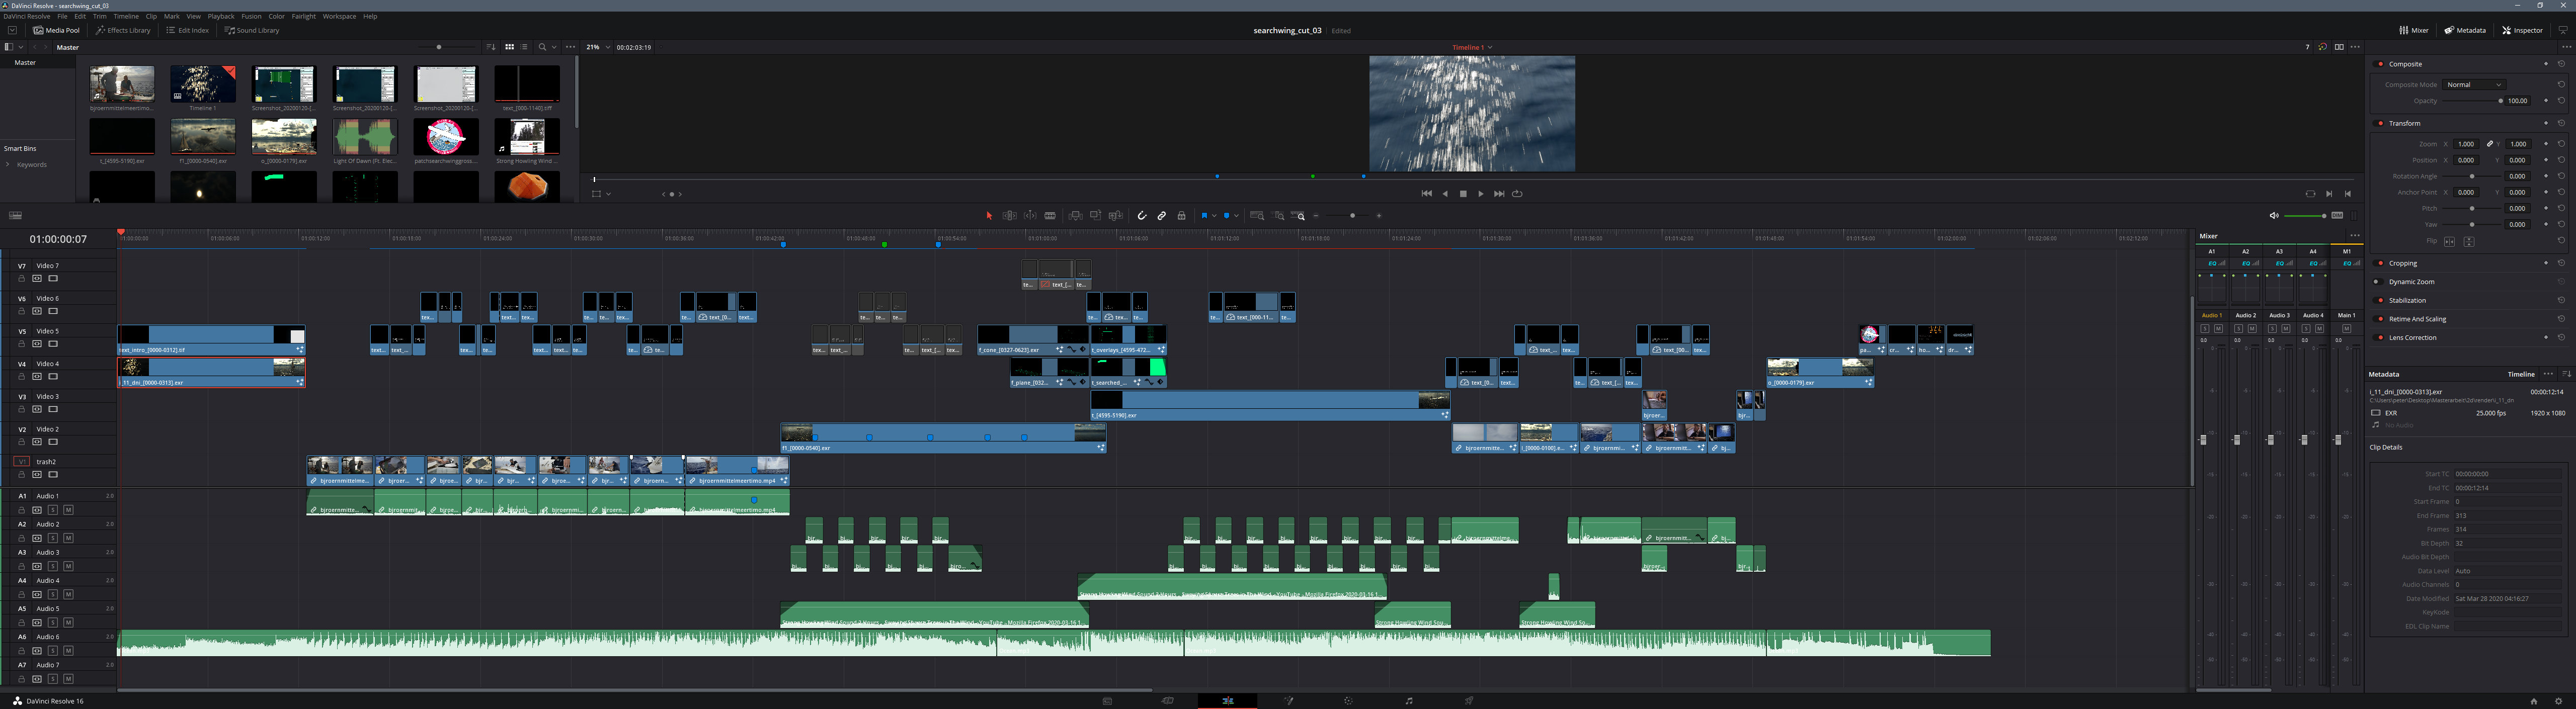
\includegraphics[width=\textwidth]{gfx/post/resolve2.jpg}
\caption{}
\label{resolve2}
\end{center}
\end{figure}

\section{Bauchbinden}
\label{sec:bauchbinden}

Die Texte für die Bauchbinden wurden in Blender erstellt. Der Grund ist, dass das gleichzeitige verschwinden von zwei Texten über unabhängige Masken konnte hier einfacher realisiert werden. Eine schräge Darstellung der Masken ist in \autoref{out2} abgebildet. Hierfür wurde eine Vorlage programmiert, welche für jeden neuen Text wiederholt wurde (siehe \autoref{out}).\\
Zwar wird hier wieder in Blender eine Bildsequenz erstellt, welche in das Schnittprogramm geladen wird -- trotzdem wird dieser Teil zur Nachbearbeitung des eigentlichen Filmmaterials gezählt.

\begin{figure}[H]
\begin{center}
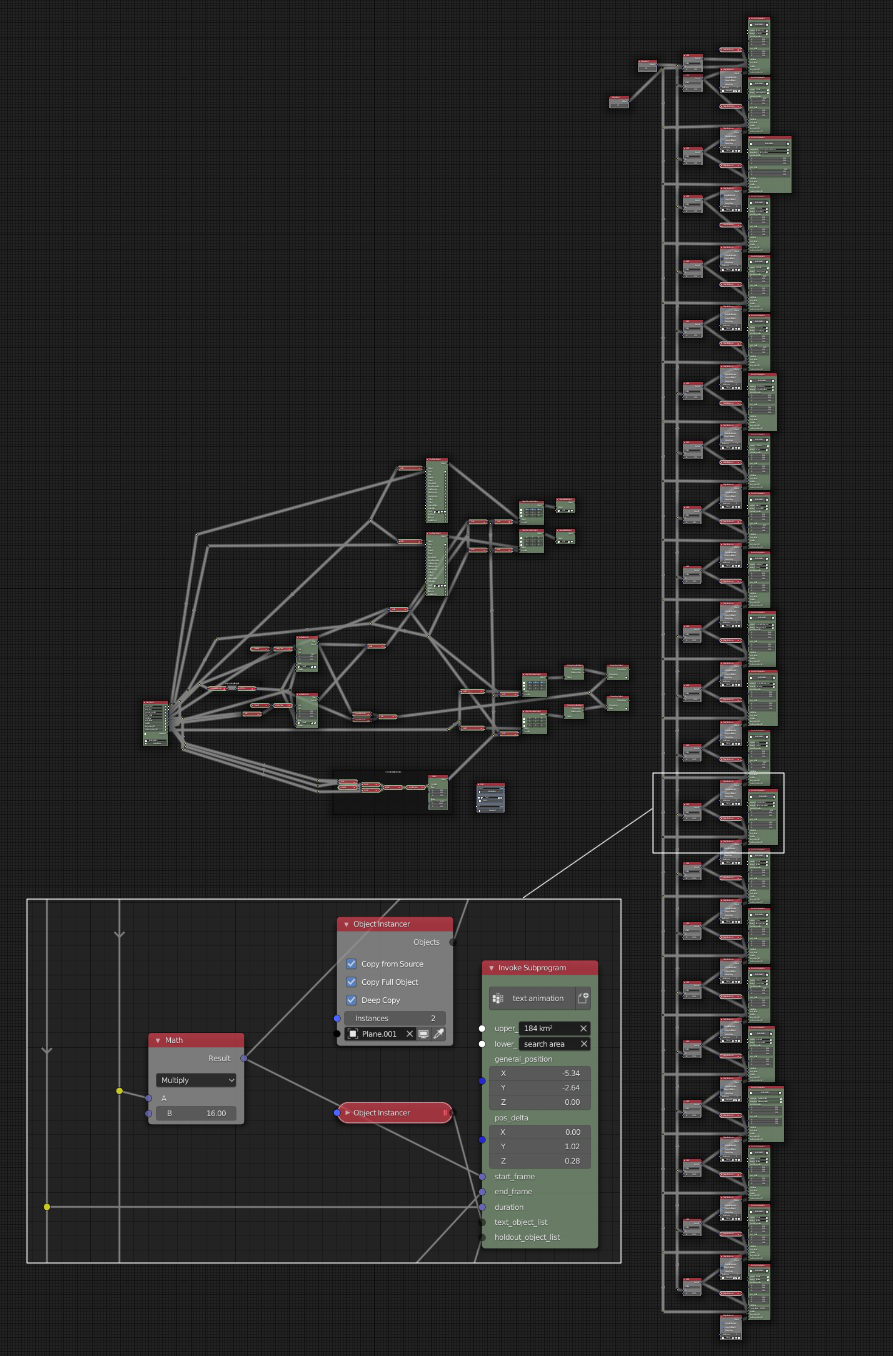
\includegraphics[width=\textwidth]{gfx/post/call-out.jpg}
\caption{Programmierte Vorlagen für die Bachbinden}
\label{out}
\end{center}
\end{figure}

\begin{figure}[H]
\begin{center}
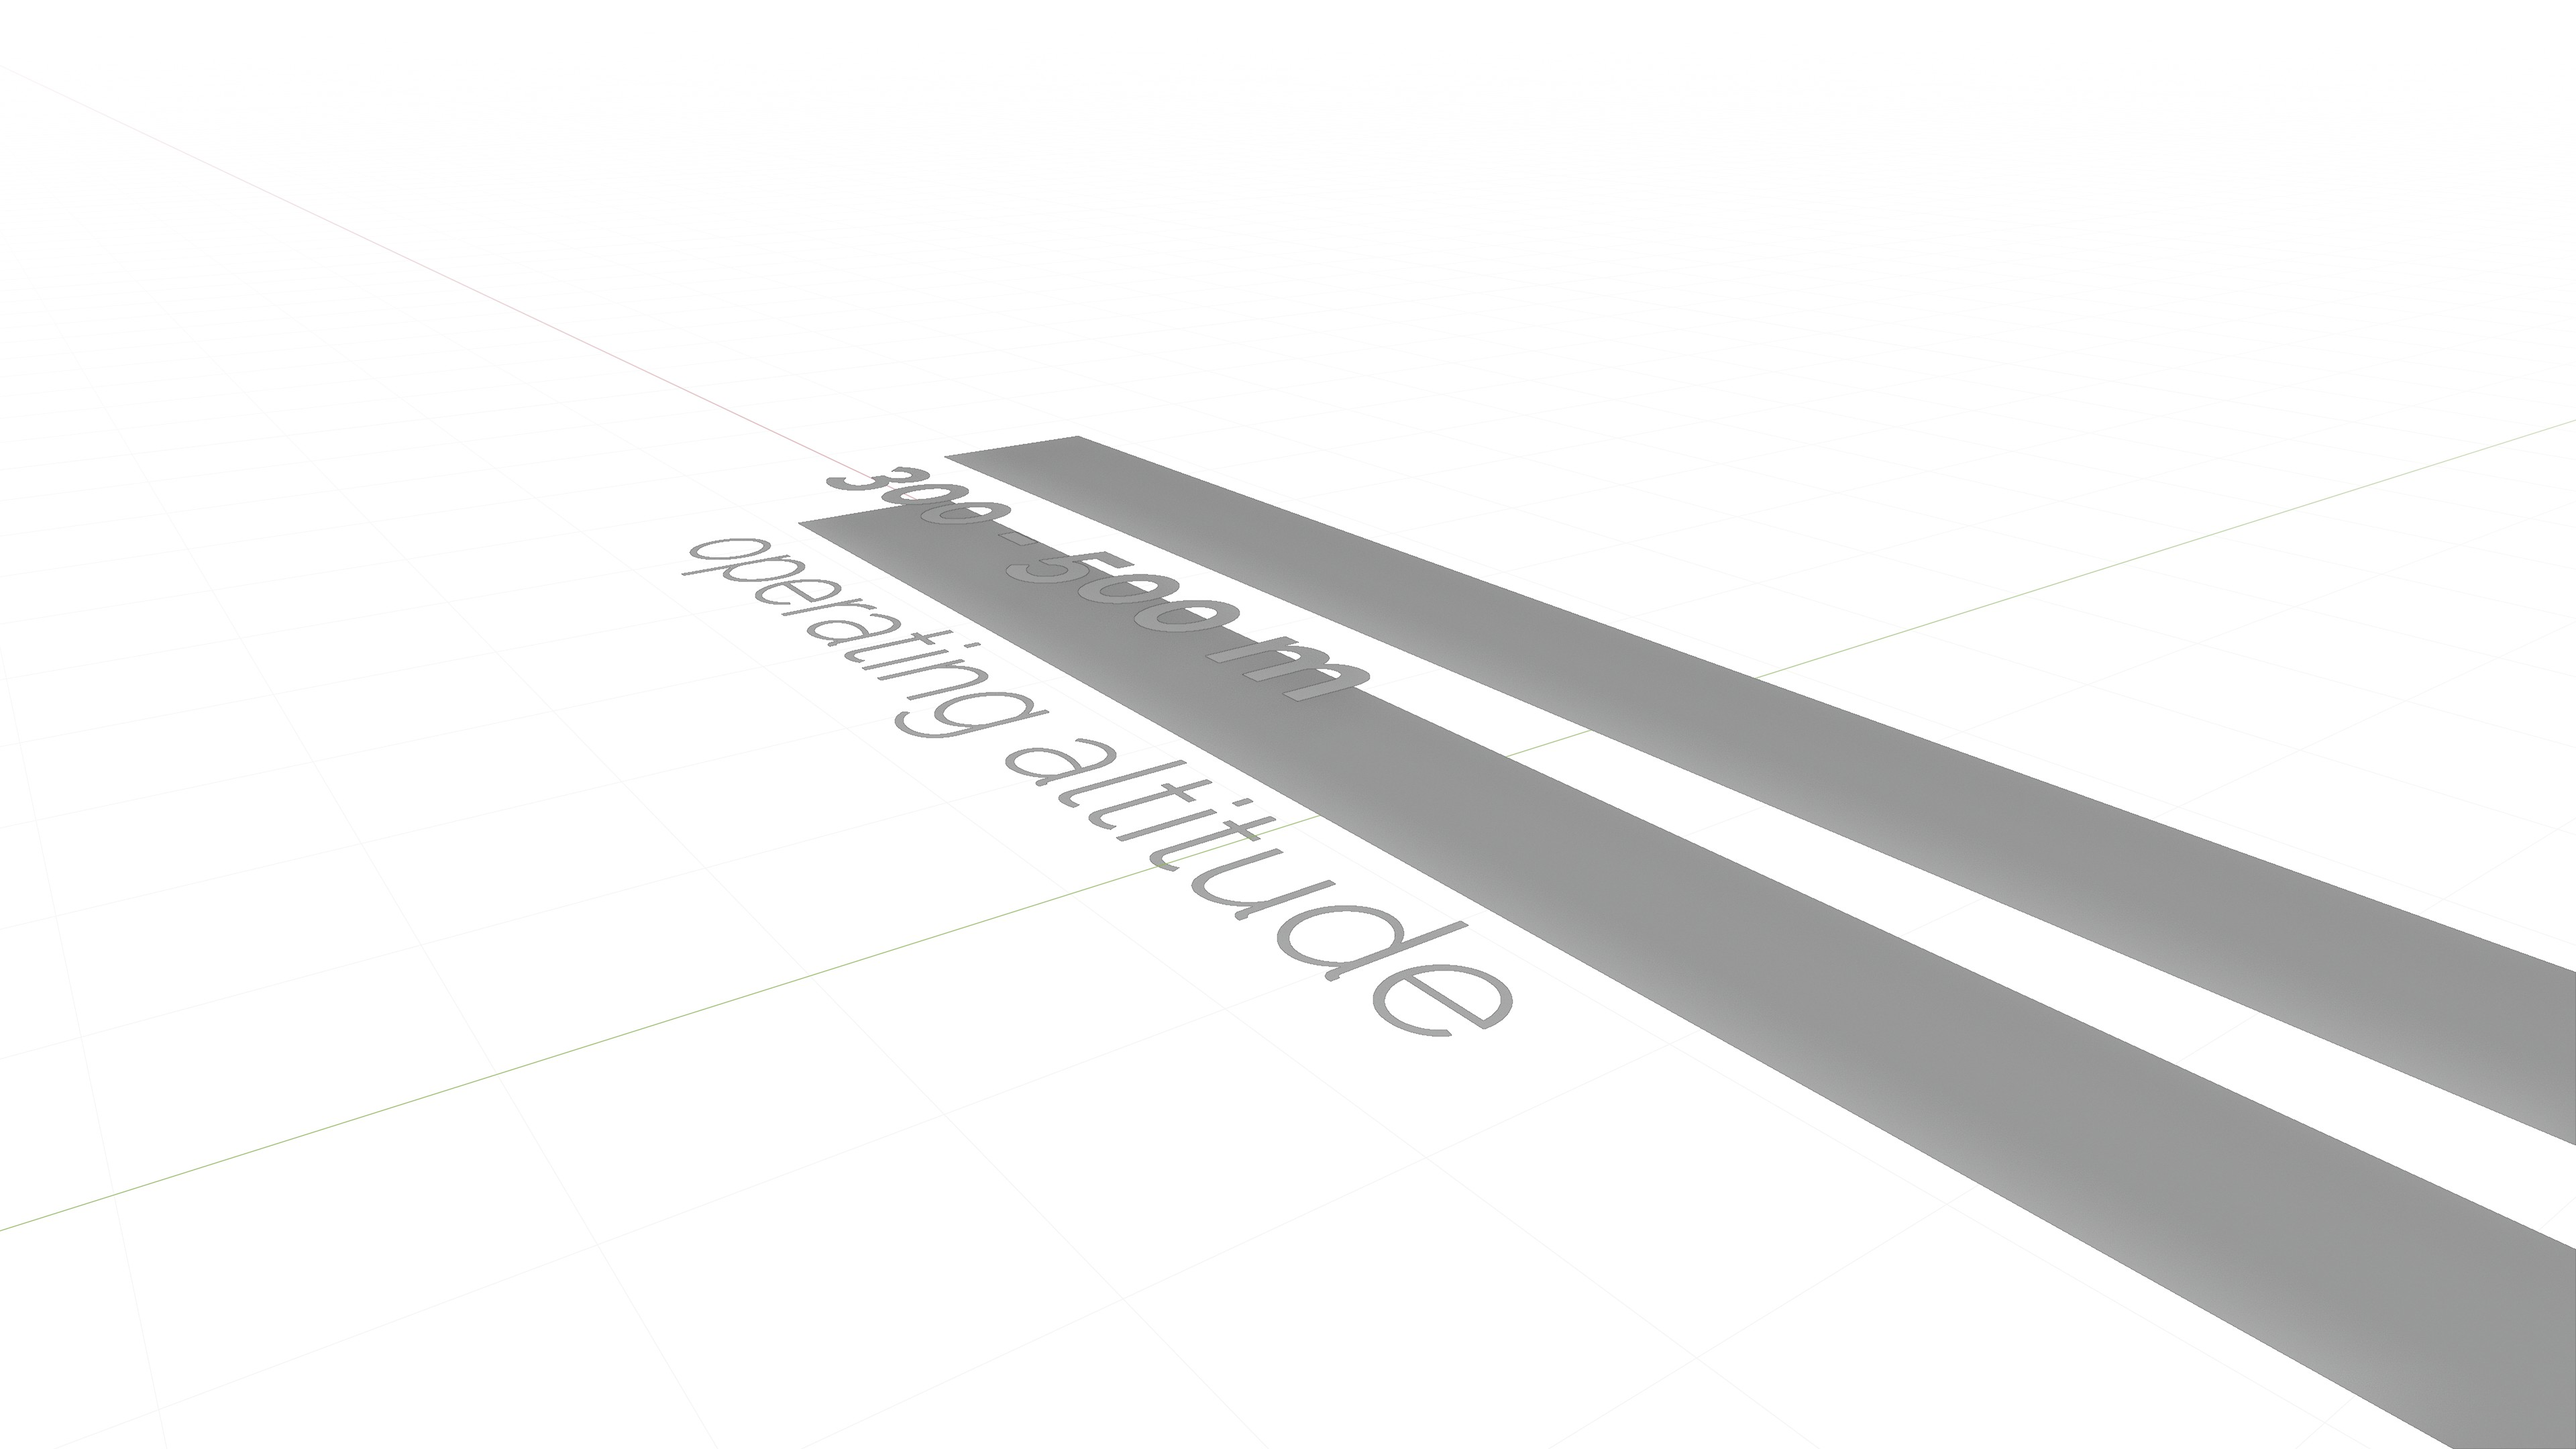
\includegraphics[width=\textwidth]{gfx/post/call-out2.jpg}
\caption{Schräge Ansicht der Masken für die Bachbinden}
\label{out2}
\end{center}
\end{figure}

Damit der Text der Bauchbinden besser lesbar ist, wurden diese mit einem Rechteck hinterlegt, welches die Optik von satiniertem Glas hat. Dies wurde mit einem Unschärfe-Filter mit einer rechteckigen Maske realisiert. Dieser Filter musste auf alle Ebenen angewendet werden, sodass separat gerenderte Filmteile ebenfalls vom Filter betroffen werden.

\begin{figure}[H]
\begin{center}
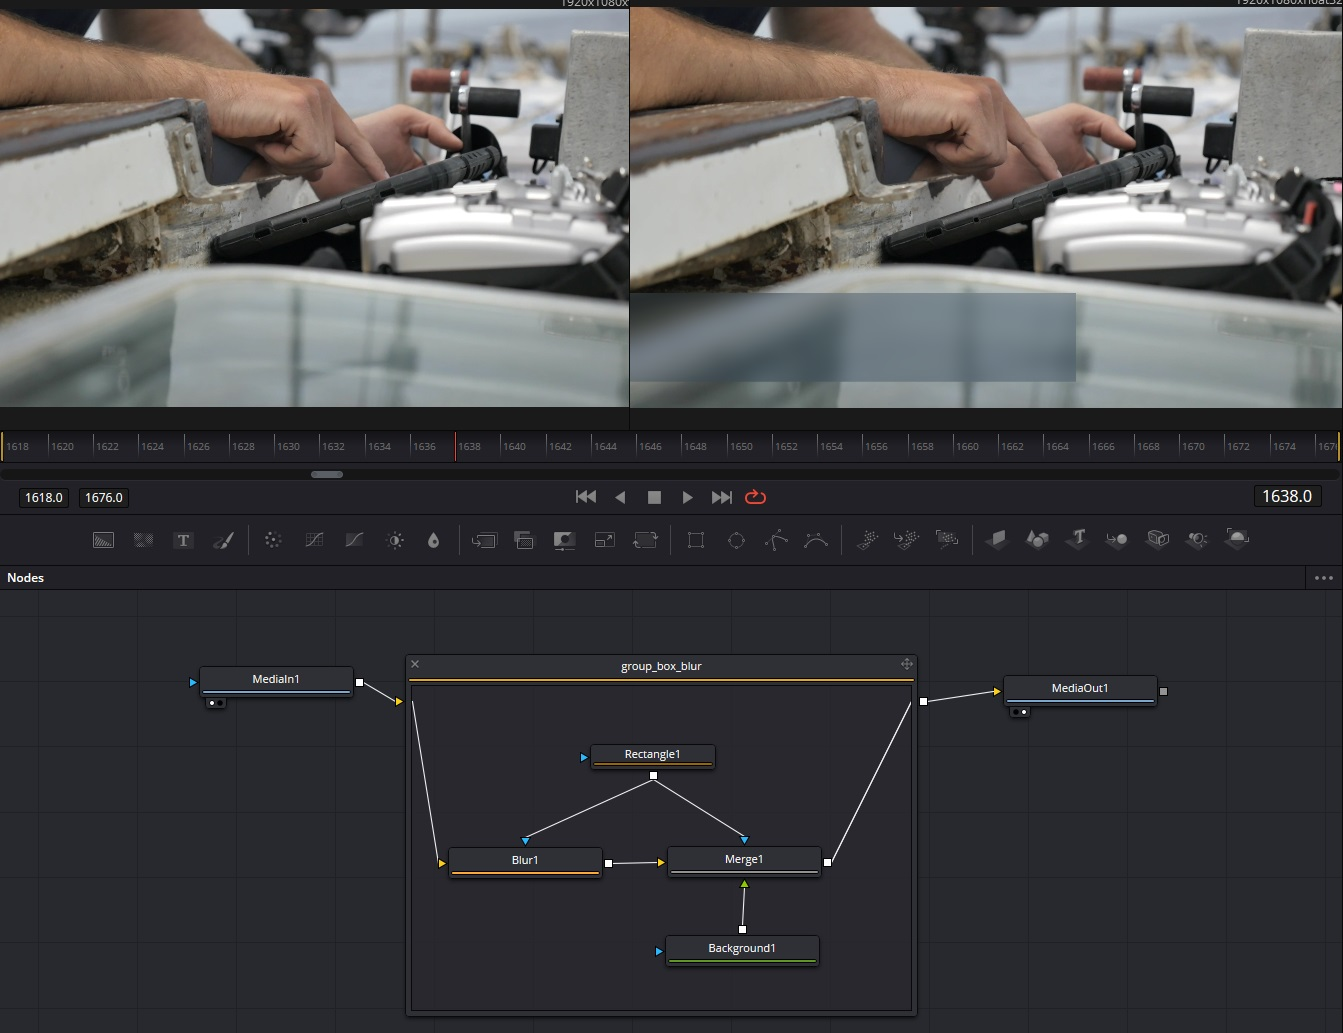
\includegraphics[width=\textwidth]{gfx/post/resolve3.jpg}
\caption{}
\label{resolve3}
\end{center}
\end{figure}

\section{Matchmoving}

\begin{figure}[H]
\begin{center}
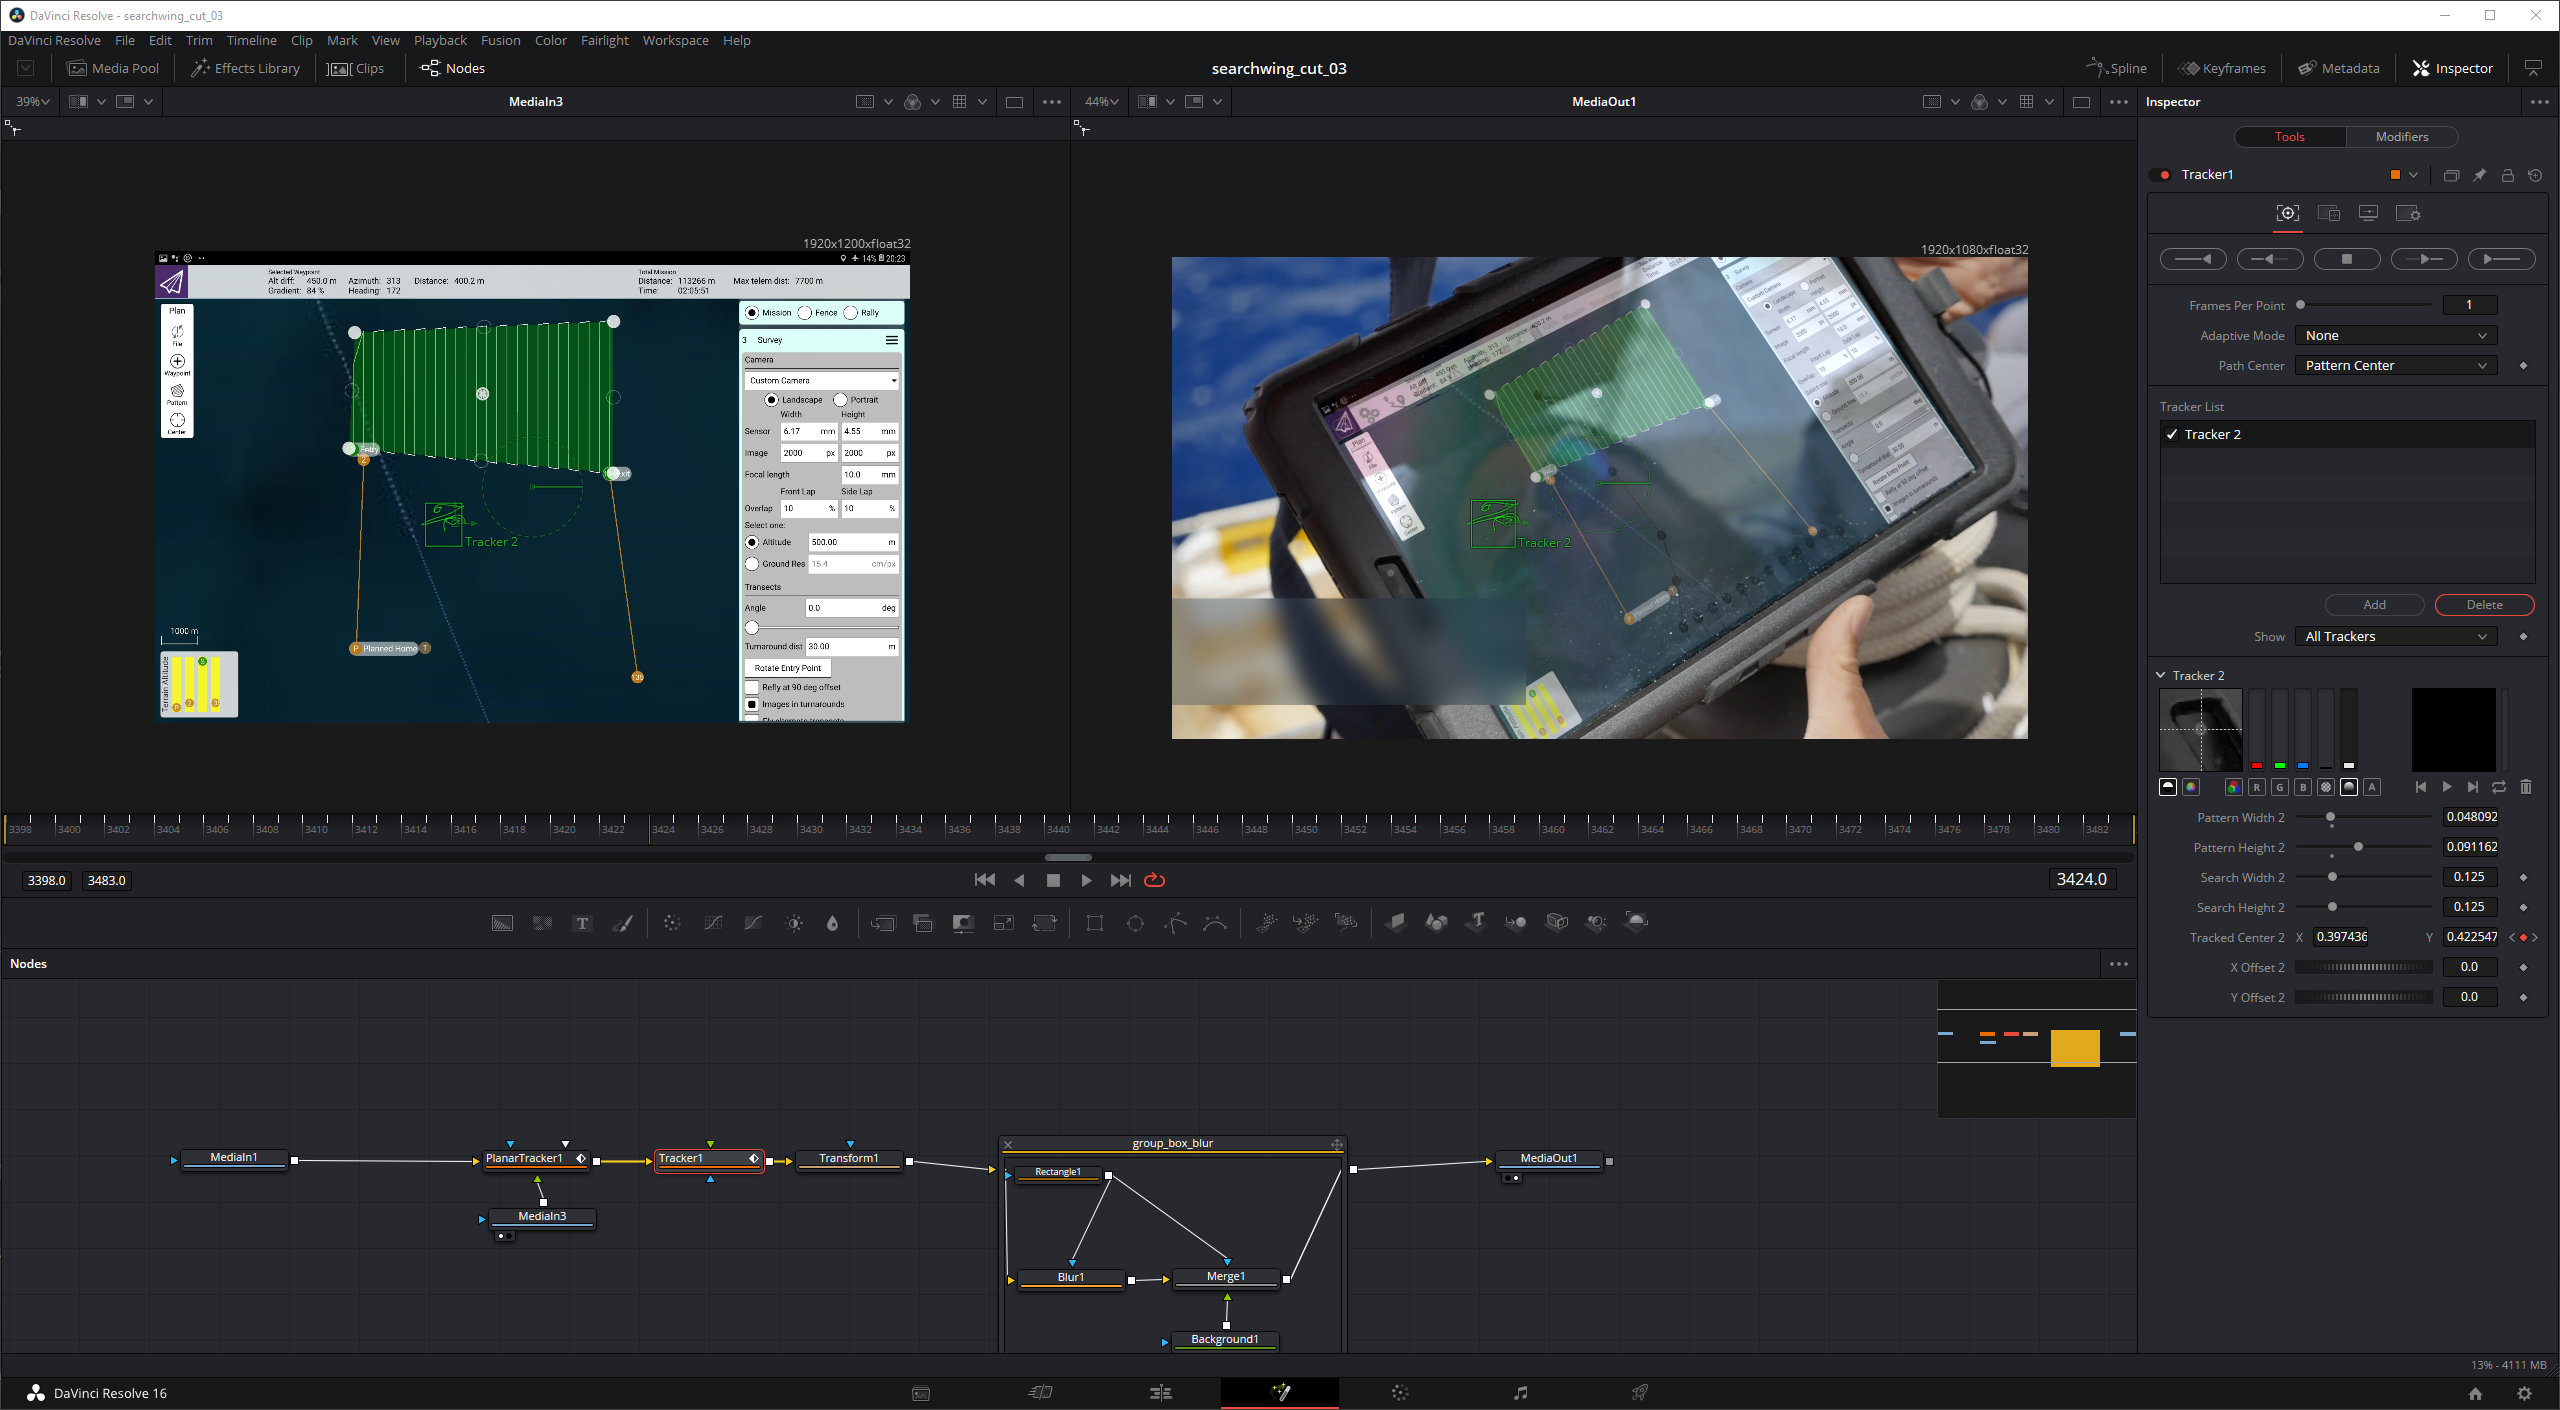
\includegraphics[width=\textwidth]{gfx/post/resolve9.jpg}
\caption{Matchmoving in der Tablet Aufnahme}
\label{resolve8}
\end{center}
\end{figure}

Das Matchmoving bezeichnet das rekonstruieren von Bewegung aus gefilmten Videomaterial. Dies wird erreicht, indem markante Punkte verfolgt werden, und anschließend aus der Bewegung dieser die Bewegung eines Objektes oder der Kamera rekonstruiert wird. \footfullcite{matchmoving}\\
In der ersten Szene, in der das Tablet sichtbar ist, wurde der Bildschirminhalt mit einem Screenshot ersetzt, da aufgrund der hellen Umgebung der Inhalt nicht gut sichtbar war. Weiterhin wurden hier mithilfe von Matchmoving ebenfalls die Bewegungen der Kamera reduziert, damit der Bildschirminhalt noch besser sichtbar ist. Ein Screenshot dieser Szene in Bearbeitung ist in \autoref{resolve8} sichtbar.\\

\begin{figure}[H]
\begin{center}
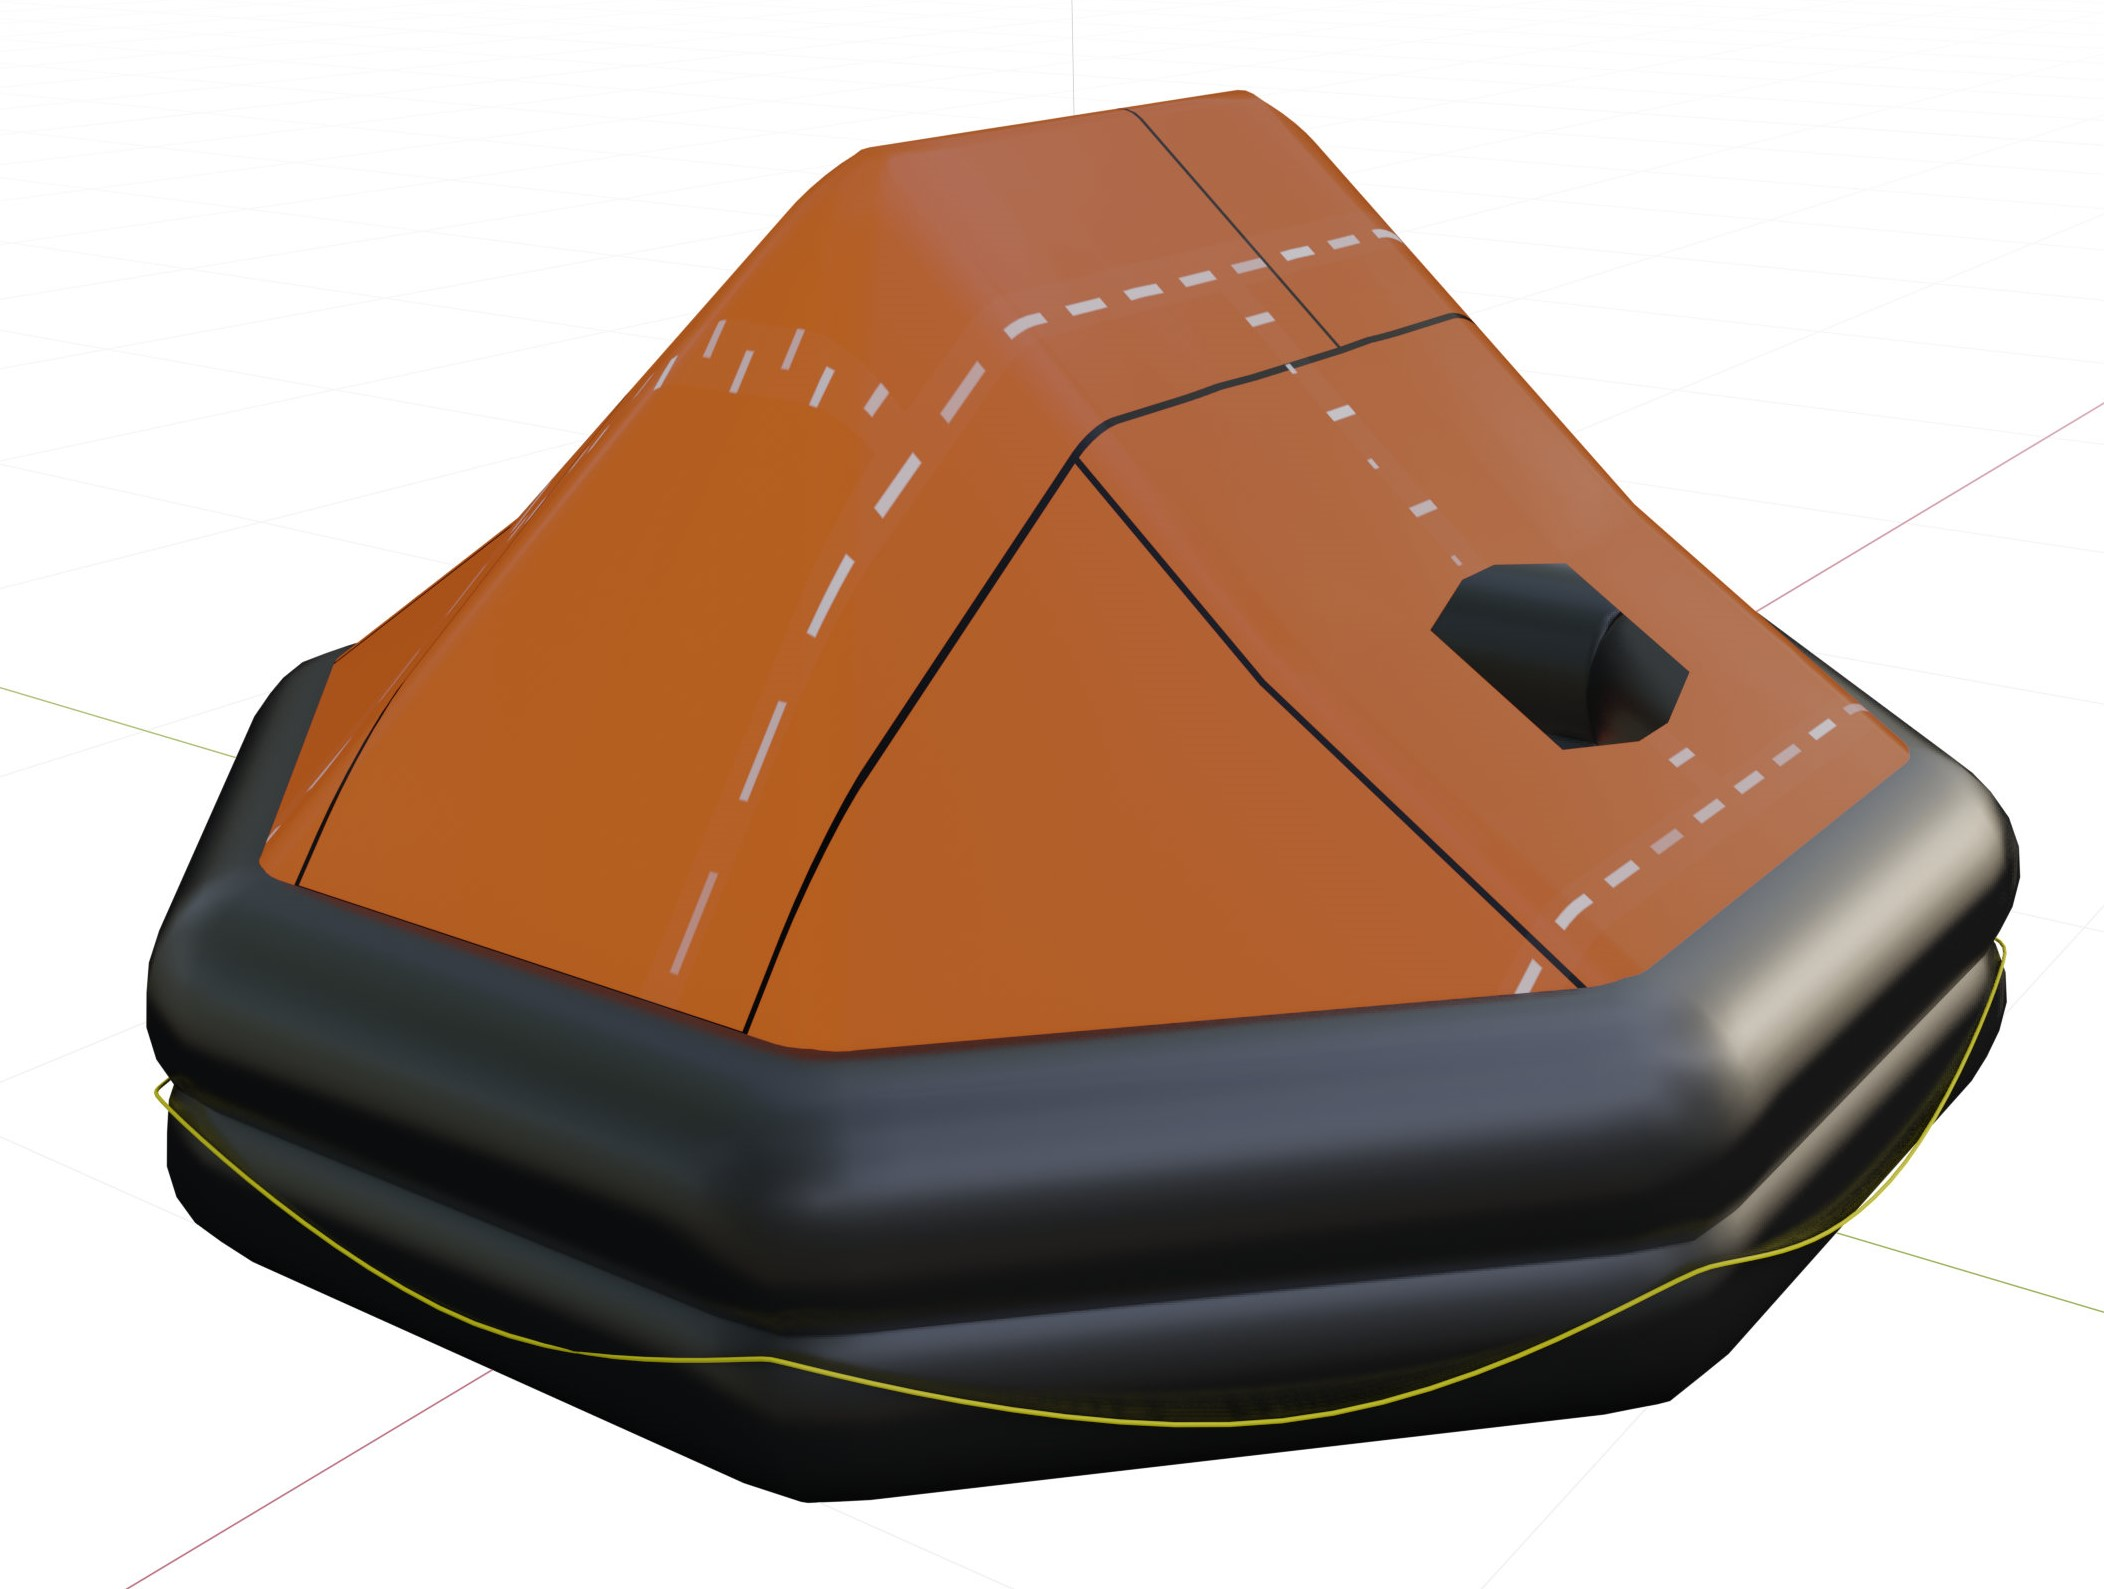
\includegraphics[width=\textwidth]{gfx/prod/boat/liferaft1.jpg}
\caption{Modell des Rettungsfloßes}
\label{liferaft1}
\end{center}
\end{figure}

Mit derselben Technik wurde ebenfalls in der Aufnahme, in der die Drohnenaufnahmen am Laptop analysiert werden, ein Rettungsfloß eingefügt. Hierzu wurde zunächst das Modell eines Rettungsfloßes erstellt (siehe \autoref{liferaft1}), dessen Bild hier eingefügt wurde (siehe \autoref{resolve10}).

\begin{figure}[H]
\begin{center}
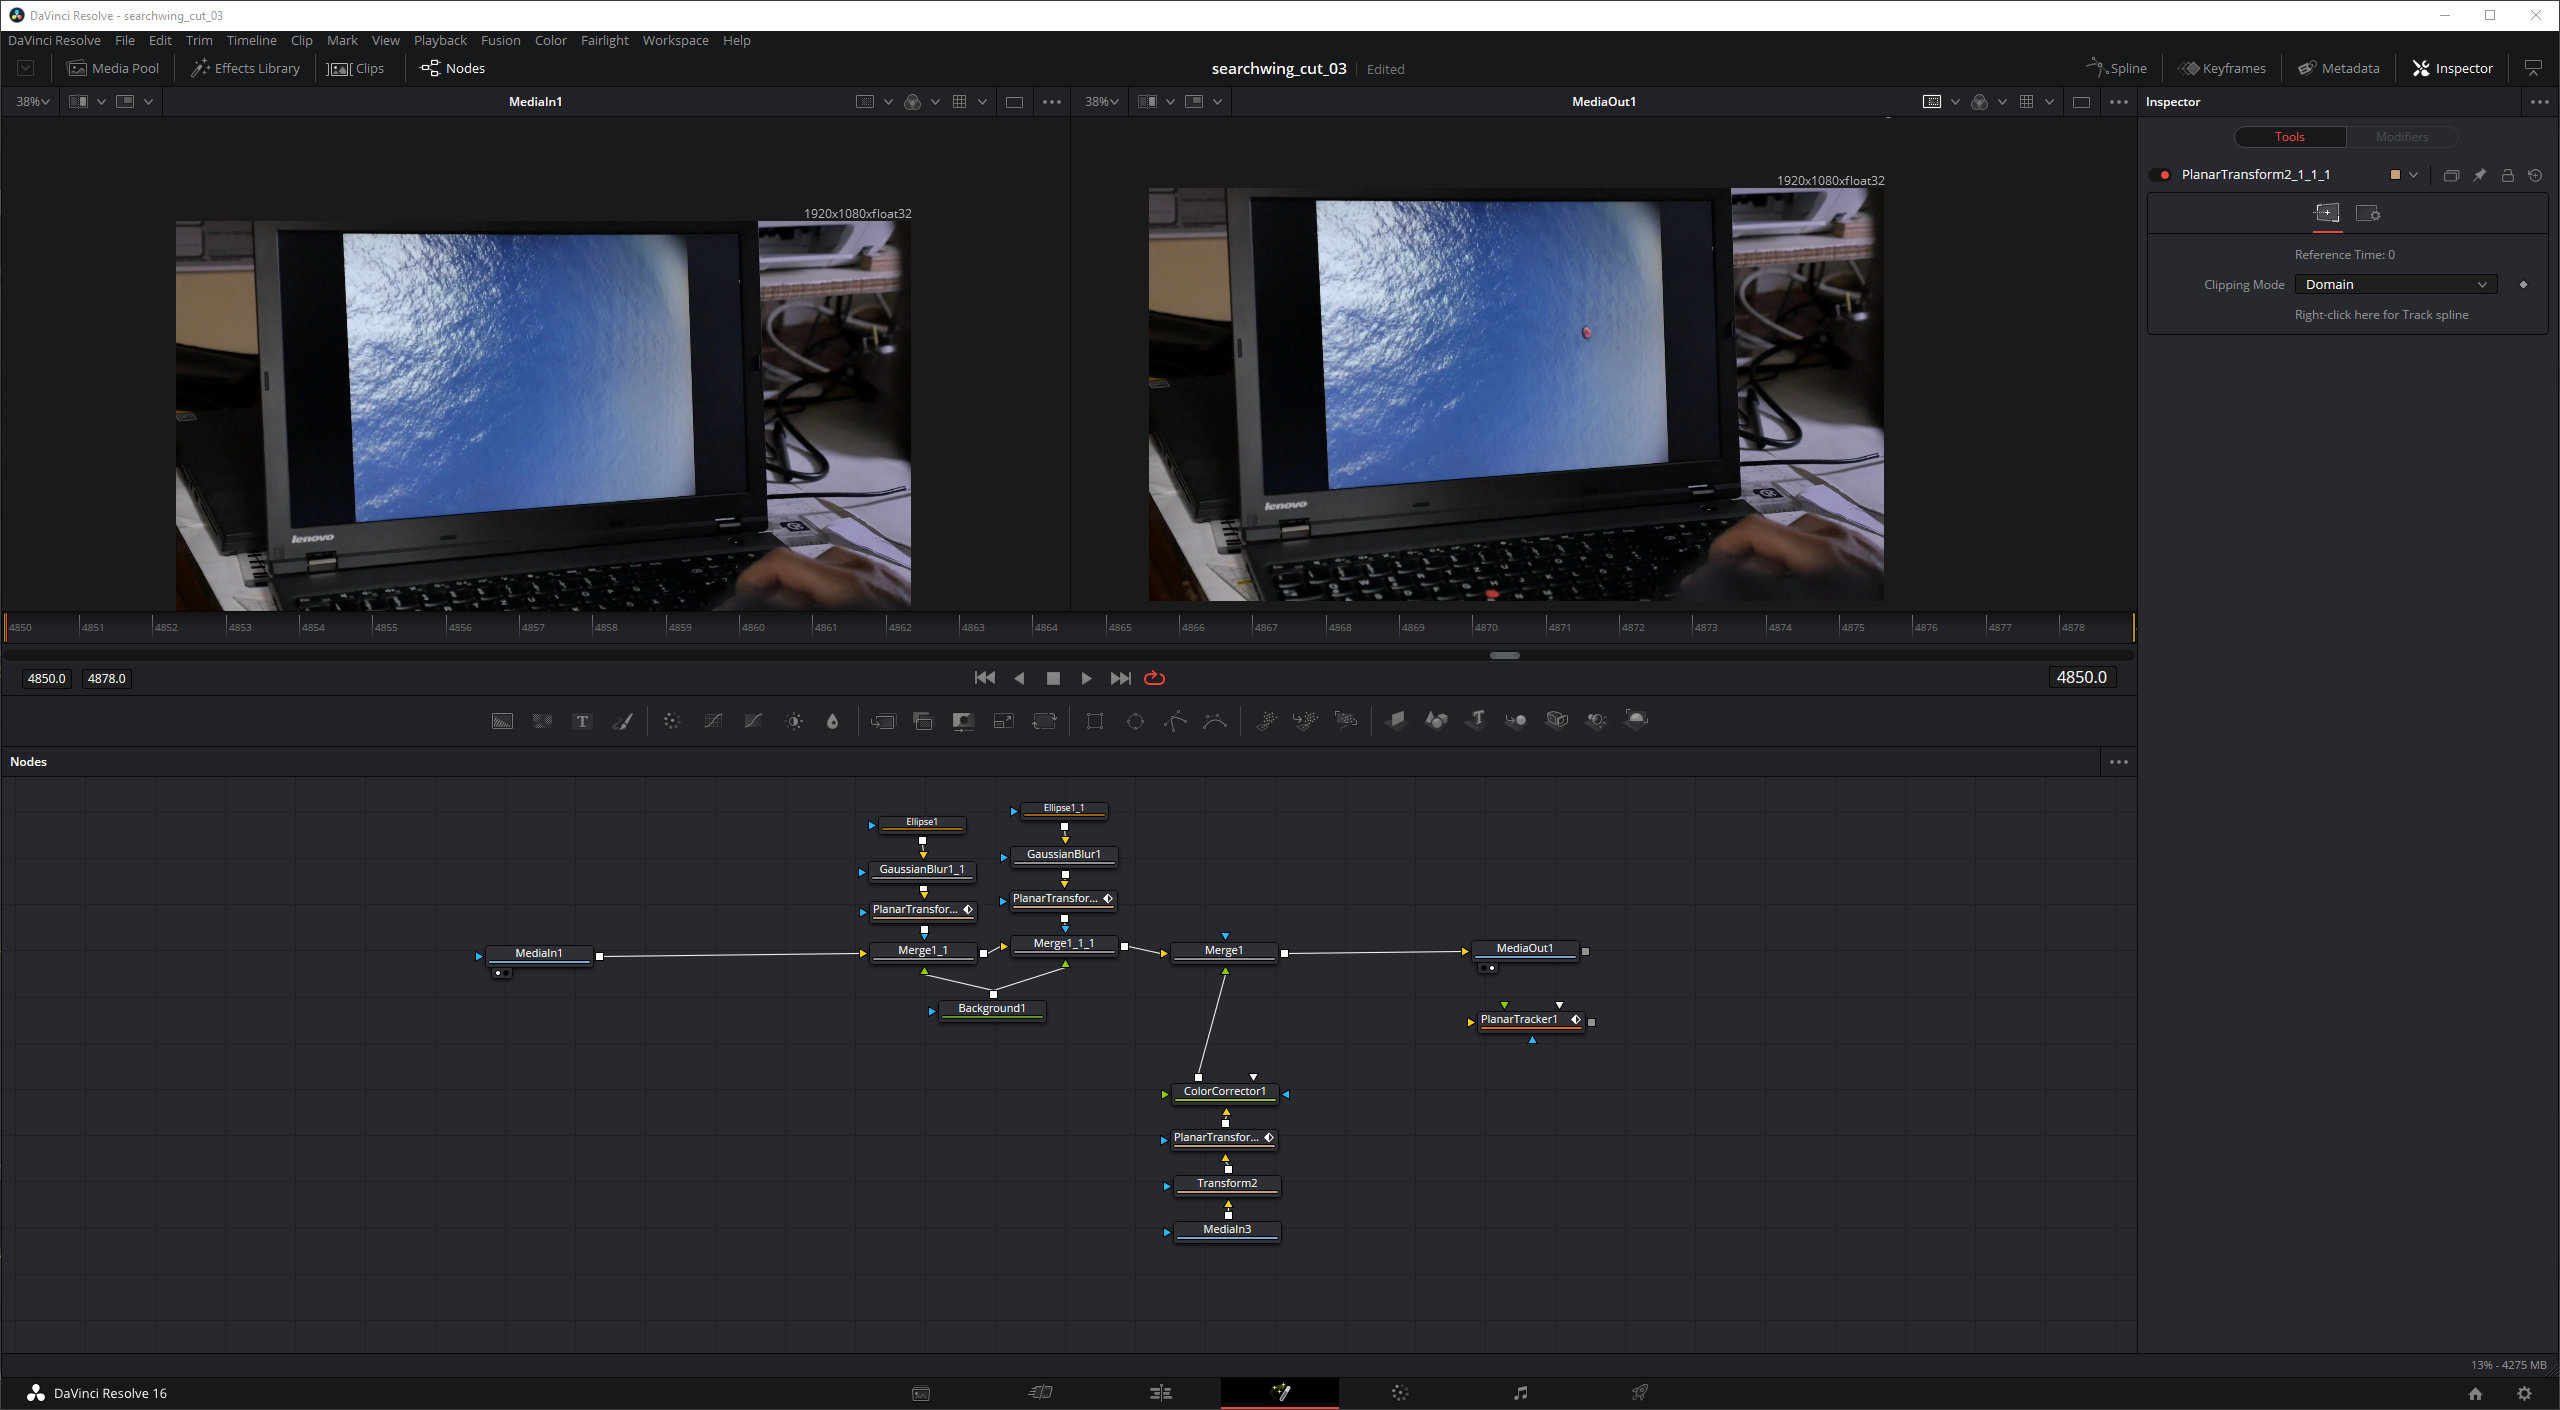
\includegraphics[width=\textwidth]{gfx/post/resolve10.jpg}
\caption{Workflow beim Einsetzen des Rettungsfloßes}
\label{resolve10}
\end{center}
\end{figure}

\begin{figure}[H]
\begin{center}
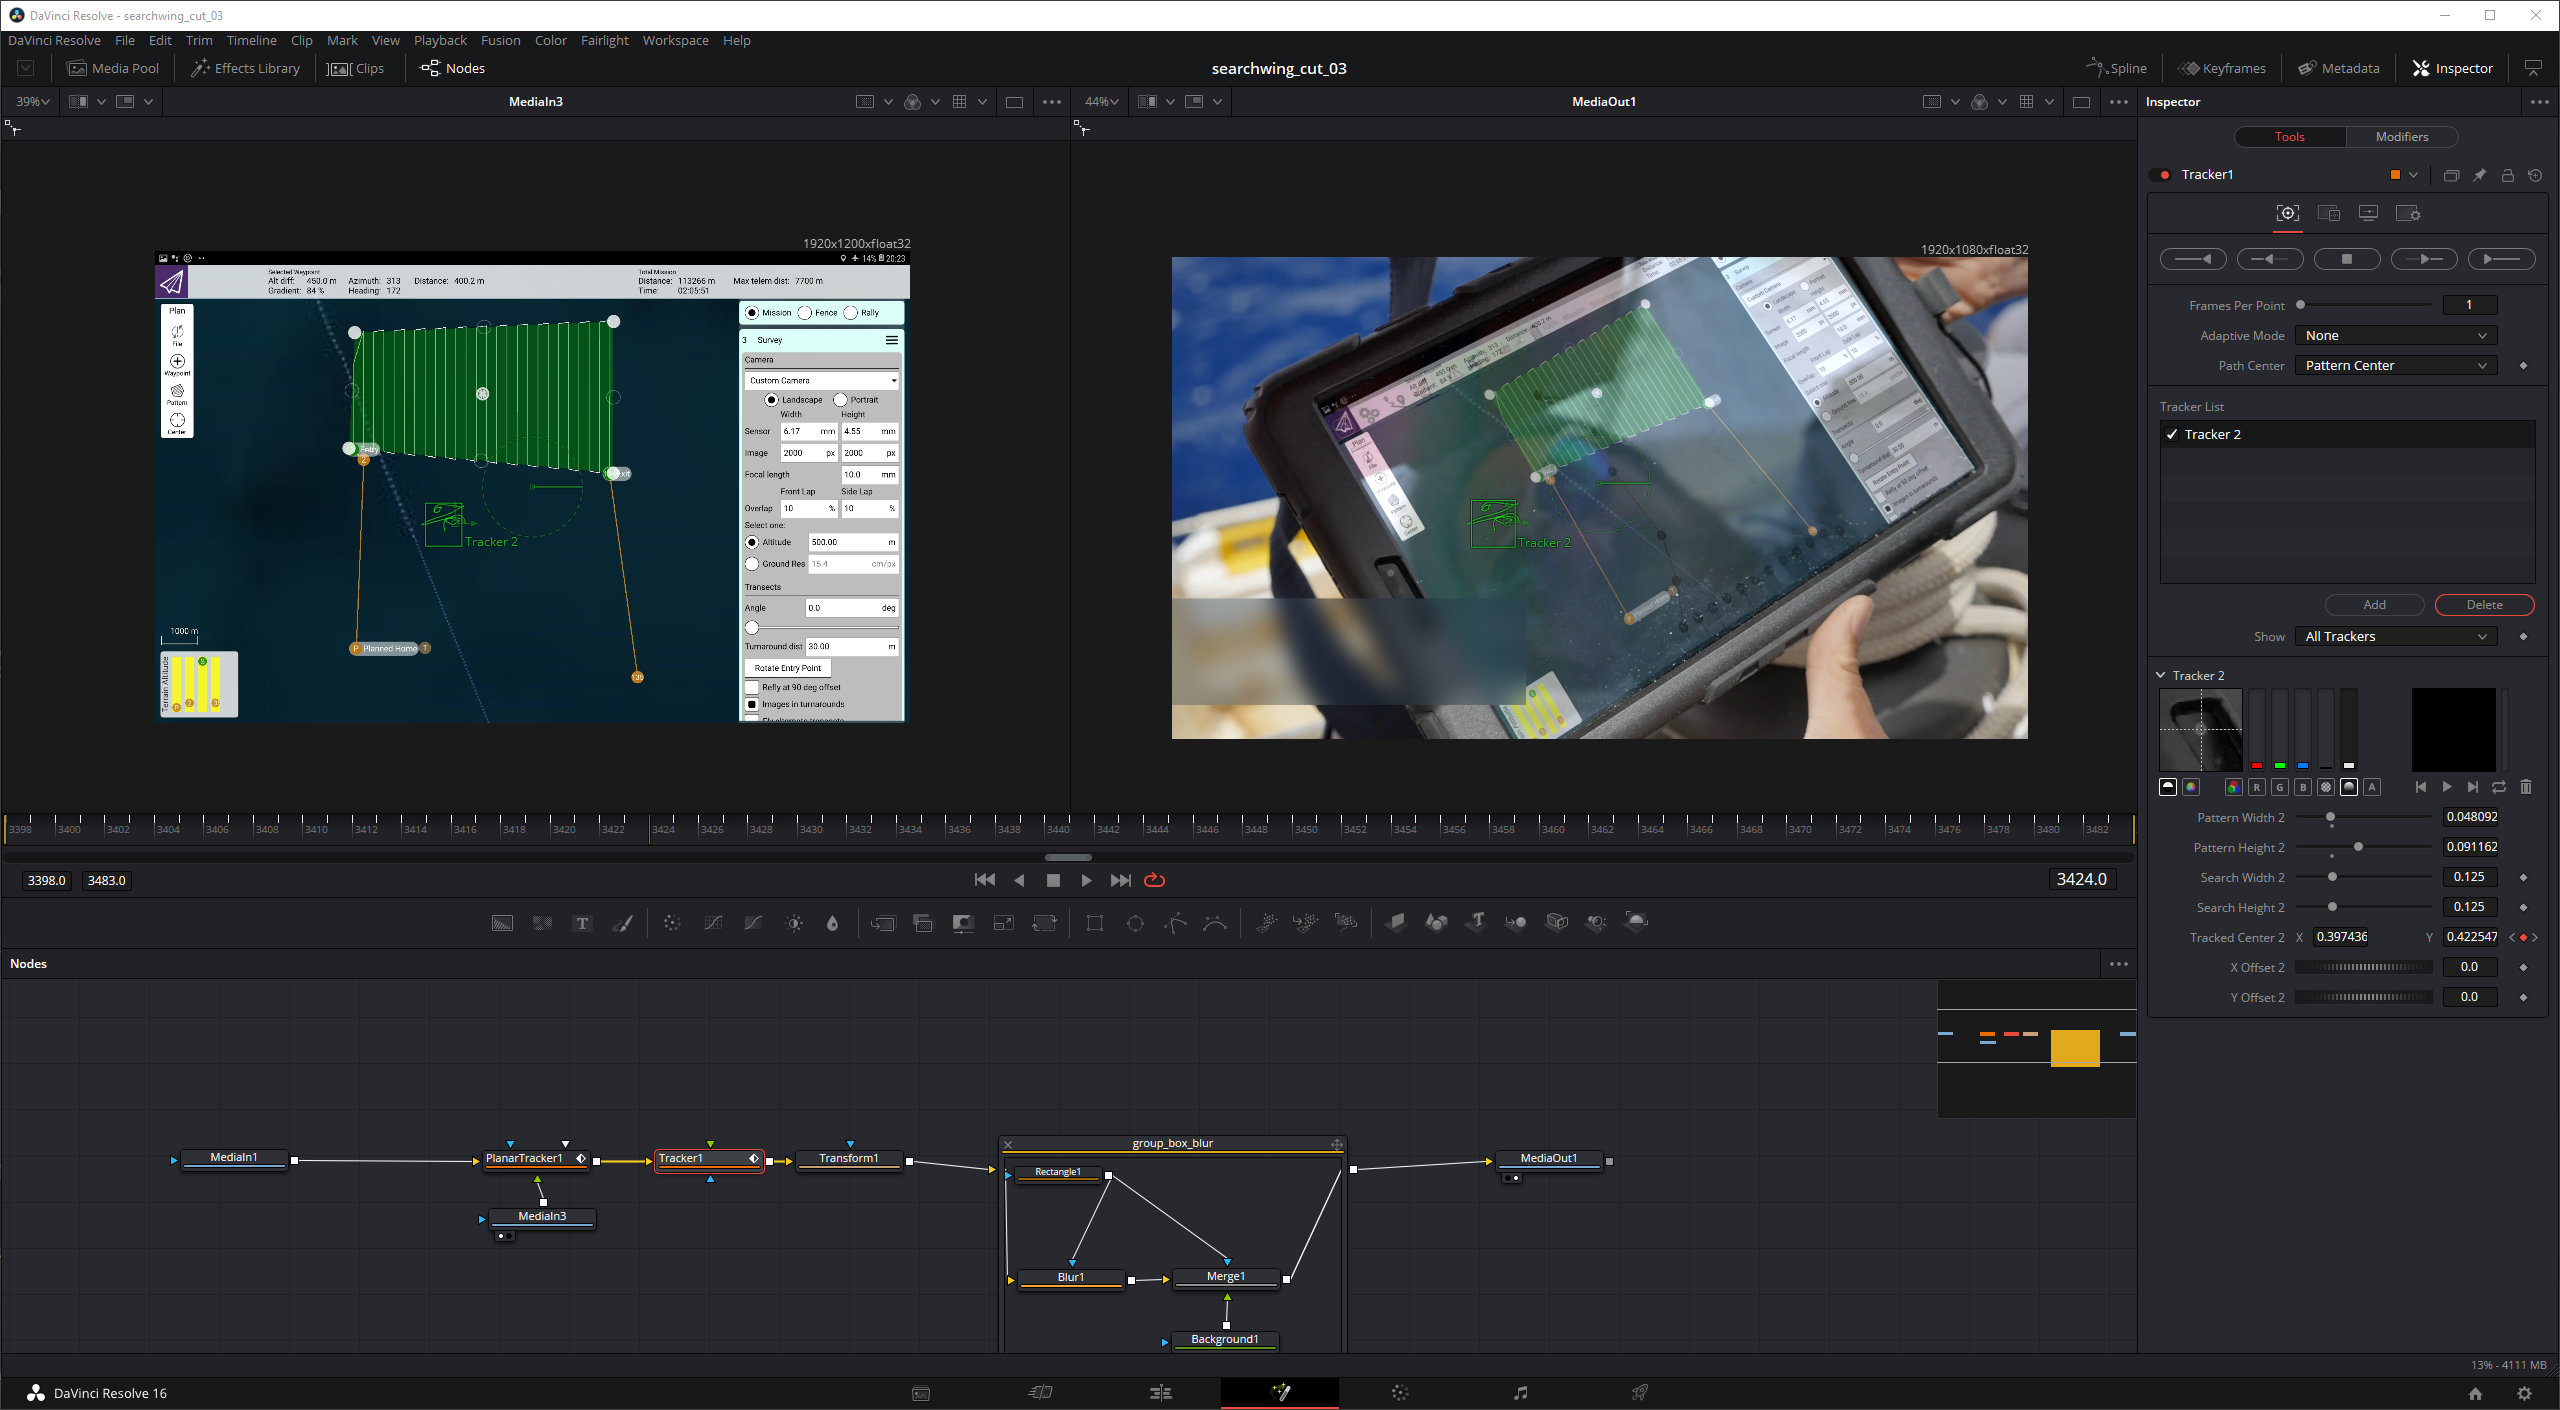
\includegraphics[width=\textwidth]{gfx/post/resolve9.jpg}
\caption{}
\label{resolve9}
\end{center}
\end{figure}

\section{Farbkorrektur}


bei radiowellen war z.b. wichtig, dass der farbraum filmic erst angewendet wird, nachdem die wellen auf das flugzeug gelegt wurden. ansonsten ausbrennen oder nicht ausnutzen des farbraumes


Anpassen über weißpunkt
Viel Potenzial übrig gewesen, da in openExr gerendert wurde.
dies war der zweite vorteil von exr dateien gegenüber einem klassischen dateiformat, wie bspw. jpg

davor aber noch anwenden von ocio color space wichtig, da open exr immer linear ohne farbraum ist
--> hinweis auf resolve3.jpg



\begin{figure}[H]
\begin{center}
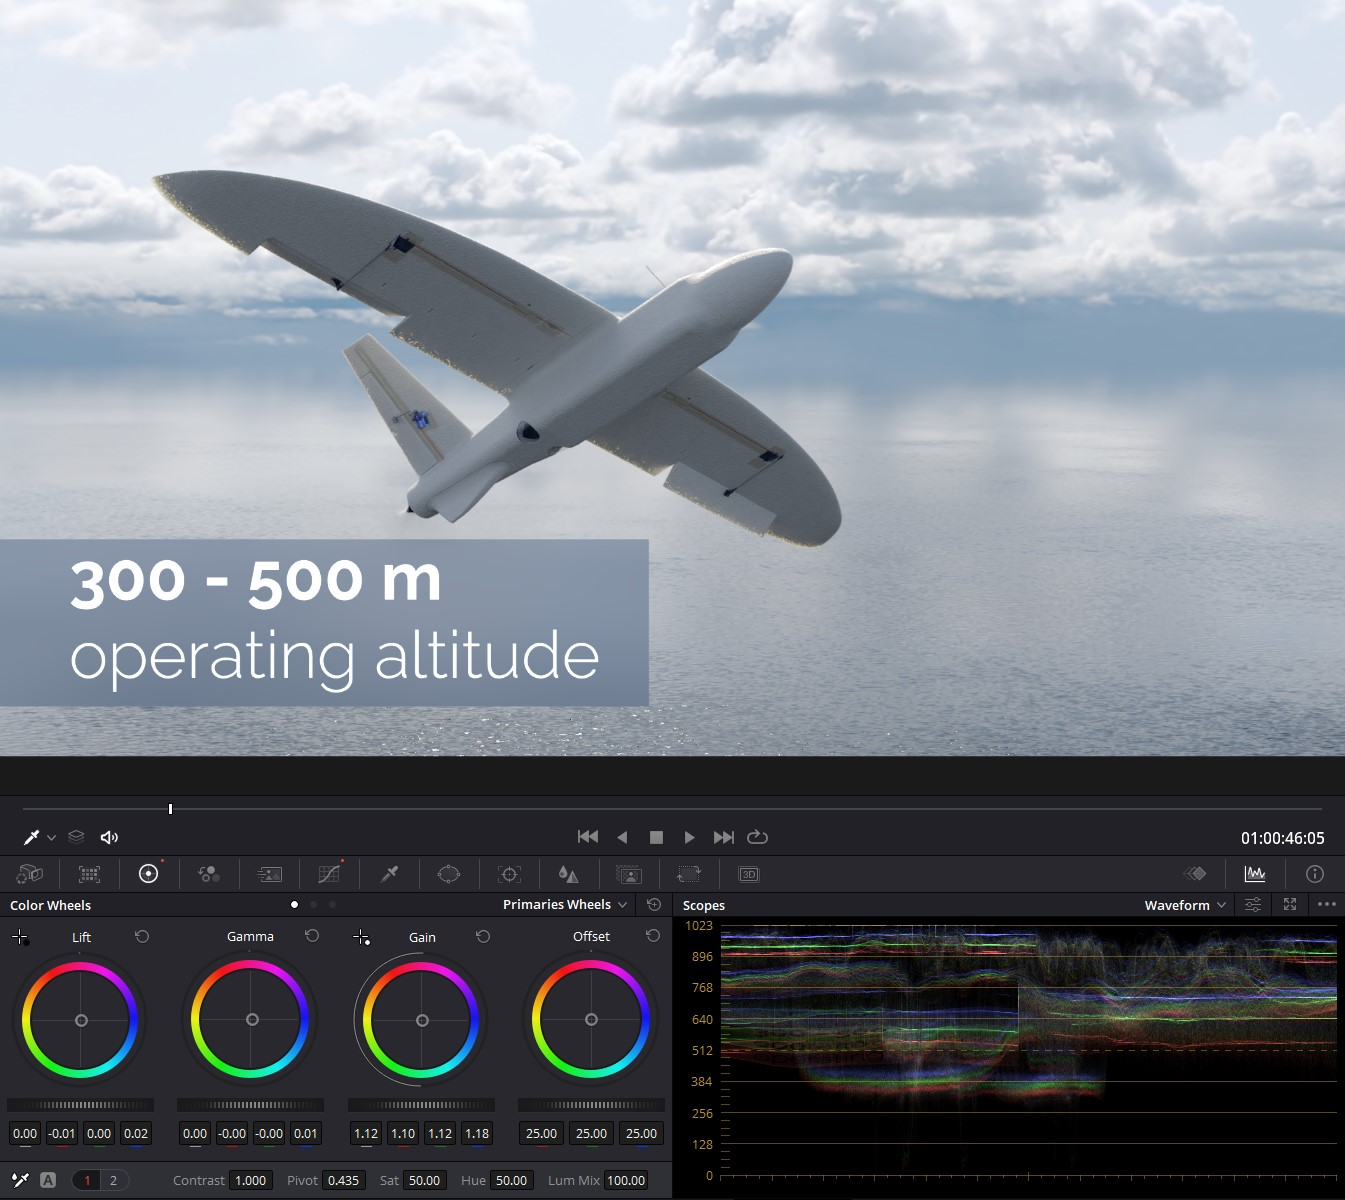
\includegraphics[width=\textwidth]{gfx/post/resolve7.jpg}
\caption{}
\label{resolve7}
\end{center}
\end{figure}

\section{Audio}

musik wurde thbd ocean entschieden
passend geschnitten. eckpunkte waren hierbei der Anfang des Filmes, das Ende des Filmes.
daher wurde zuerst der titel in der mitte zerschnitten
der schnitt wurde anschließend so gewählt, dass er an einer passenden stelle ist
konkret heißt das, dass der schnitt möglichst unaufällig bei 0:56 der schnitt gesetzt wurde
ziel war damit, dass bei dem stärkeren visuellen wechsel von der seitenansicht des sichtkegels in die draufsicht die musik sich ändert
motor sample wurde kopiert und denn mehrfach nacheinander abgespielt. außerdem wurde der audio-ausschnitt manchmal gespiegelt, sodass es schwieriger zu erkennen ist, dass es sich wiederholt
Dass der Motorsound und die Musik dieselbe tonhöhe haben, war ein glücklicher zufall
WIndgeräusche


\begin{figure}[H]
\begin{center}
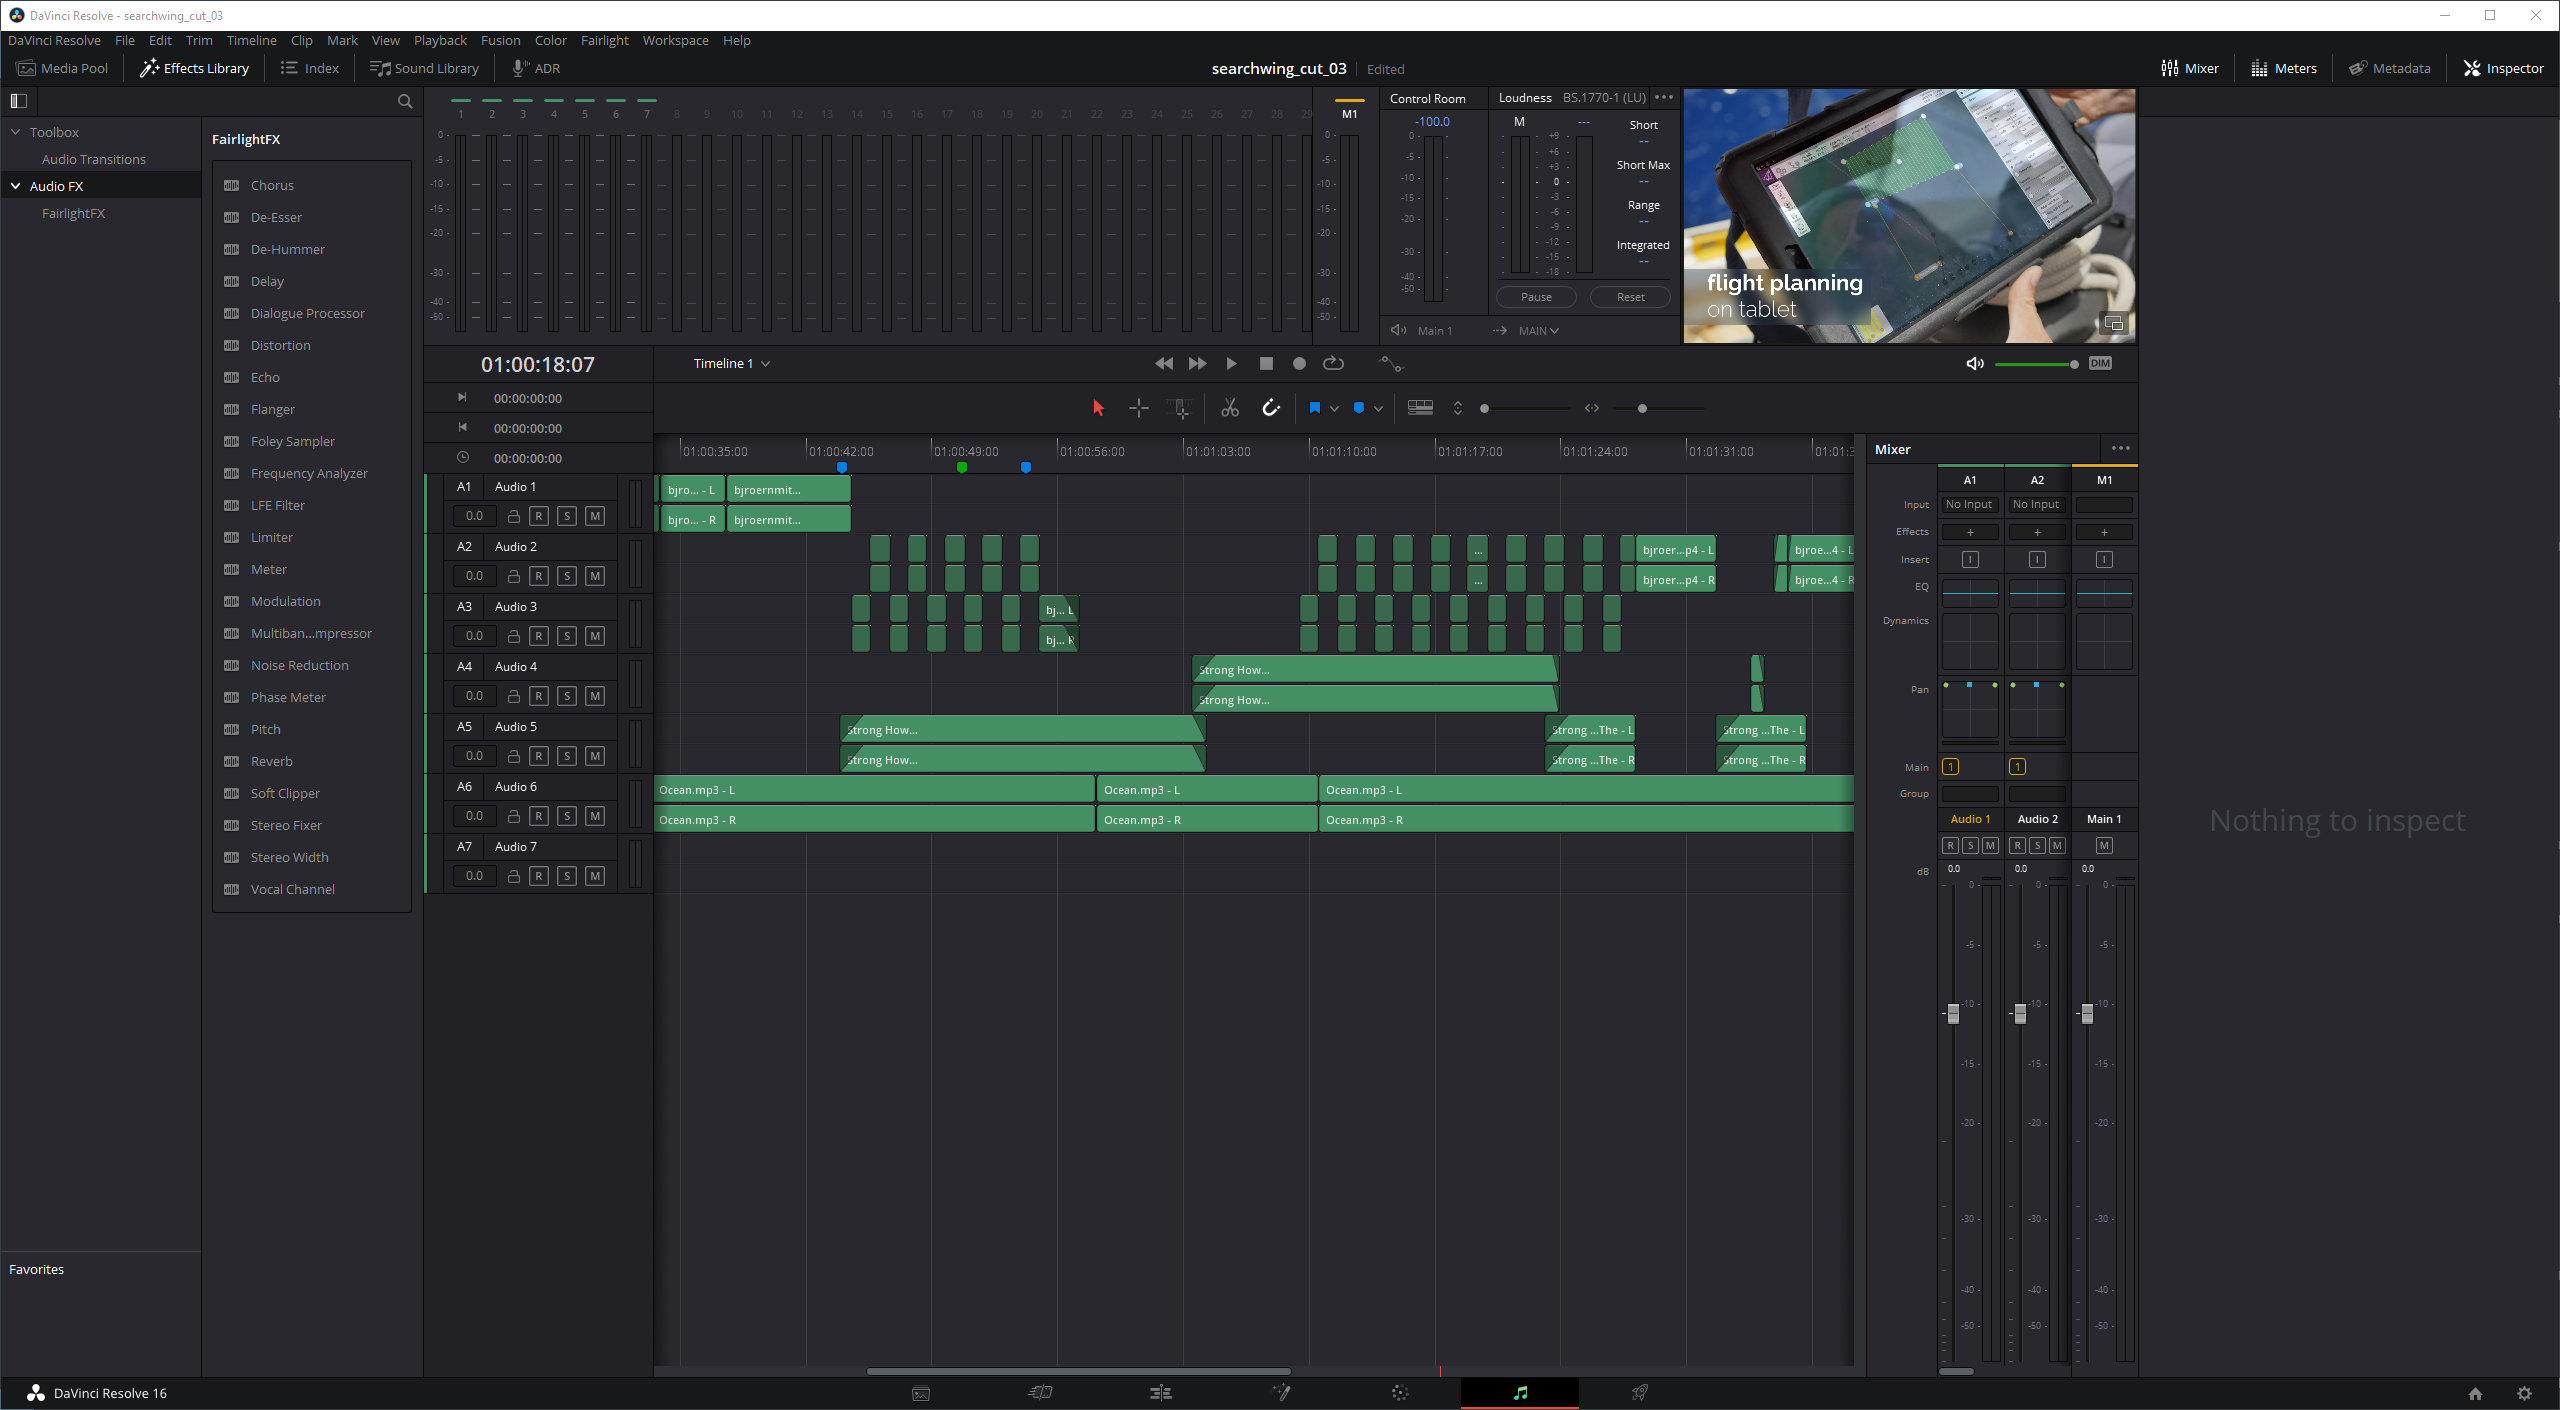
\includegraphics[width=\textwidth]{gfx/post/resolve1.jpg}
\caption{}
\label{resolve1}
\end{center}
\end{figure}

\begin{figure}[H]
\begin{center}
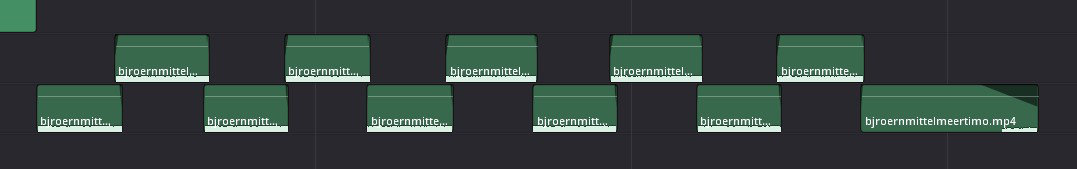
\includegraphics[width=\textwidth]{gfx/post/sample.jpg}
\caption{}
\label{sample}
\end{center}
\end{figure}